\chapter{Theoretical Approach or Different Title}

\begin{justify}
    Manual spacing between paragraphs are not permitted
\end{justify}

%%%%%%%%%%%%%%%%%%%%%%%%%%%%%%%%%%%%%%%%%%%%%%%%%%%%%%%%%%%%%%%%%%%%%%%%%%%%%%%%%%%%%%%%%%%%%%%%%%%%%%%%%%
\section{New Section Title}
\begin{justify}

    Content..........................\\
    Content..........................\\
    Content..........................\\
    Content..........................

\end{justify}

%%%%%%%%%%%%%%%%%%%%%%%%%%%%%%%%%%%%%%%%%%%%%%%%%%%%%%%%%%%%%%%%%%%%%%%%%%%%%%%%%%%%%%%%%%%%%%%%%%%%%%%%%%
\subsection{New Subsection Title – Figures}
\begin{justify}

    It's essential to take the following consideration when inserting Figures.

    \begin{itemize}[itemsep=0.5ex]
        \item Figures should be original with good resolution and do not violate copy rights, other people work must be referenced.
        \item Figure size have to be consistent through the thesis , this means unless necessary figures have to have approximately in same size.
        \item Figure abbreviation and number in text have to match the caption
        \item If the figure did not fit in the page then bring the text after and put the figure in next page.
    \end{itemize}


    \begin{figure}[H]
        \centerline{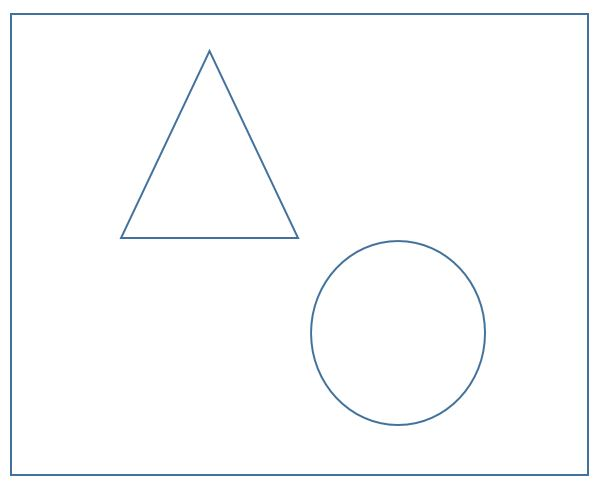
\includegraphics[width=100mm,scale=1]{figures/figure.jpg}}
        \caption{The figure caption}
        \label{fig}
    \end{figure}

\end{justify}

%%%%%%%%%%%%%%%%%%%%%%%%%%%%%%%%%%%%%%%%%%%%%%%%%%%%%%%%%%%%%%%%%%%%%%%%%%%%%%%%%%%%%%%%%%%%%%%%%%%%%%%%%%
\subsection{New Subsection Title – Tables}
\begin{justify}





% use the online editor tool to generate a table like below https://www.latex-tables.com/
\renewcommand{\arraystretch}{1.5}
\begin{table}[H]
\centering
\caption{The table caption}
\arrayrulecolor{black}
\begin{tabular}{|p{2.25cm}|p{1.75cm}|p{1.75cm}|p{7.75cm}|}
\hline
\rowcolor[rgb]{0.914,0.914,0.914} \multicolumn{1}{|c|}{{\cellcolor[rgb]{0.914,0.914,0.914}}}                                   & \multicolumn{3}{c|}{\textbf{Titles}}                                      \\
\hhline{|>{\arrayrulecolor[rgb]{0.914,0.914,0.914}}->{\arrayrulecolor{black}}---|}
\rowcolor[rgb]{0.914,0.914,0.914} \multicolumn{1}{|c|}{\multirow{-2}{*}{{\cellcolor[rgb]{0.914,0.914,0.914}}\textbf{Heading}}} & \textbf{Title1} & \textbf{Title2} & \textbf{Title3}                       \\
\hline
{\cellcolor[rgb]{0.914,0.914,0.914}}Title1                                                                                     &                 &                 & {\cellcolor[rgb]{0.965,0.965,0.965}}  \\
\hline
{\cellcolor[rgb]{0.914,0.914,0.914}}Title2                                                                                     &                 &                 &                                       \\
\hline
{\cellcolor[rgb]{0.914,0.914,0.914}}Title3                                                                                     &                 &                 &                                       \\
\hline
\end{tabular}
\end{table}


    If a table spans more than one page then the first raw (Title) should be inserted in the next page

\end{justify}

%%%%%%%%%%%%%%%%%%%%%%%%%%%%%%%%%%%%%%%%%%%%%%%%%%%%%%%%%%%%%%%%%%%%%%%%%%%%%%%%%%%%%%%%%%%%%%%%%%%%%%%%%%
\subsection{New Subsection Title – Numbering and Bullet Points}
\begin{justify}

    Four level numbering is not permitted, if needed use bullet points.\\
    Use the following style for bullet points and numbers
    \begin{itemize}
        \item Content...
        \item Content...
            \begin{itemize}
                \item Content...
                \item Content...
                    \begin{itemize}
                        \item Content...
                        \item Content...
                    \end{itemize}
                \item Content...
            \end{itemize}
        \item Content...
    \end{itemize}

    \begin{enumerate}
        \item Content...
        \item Content...
            \begin{enumerate}
                \item Content...
                \item Content...
            \end{enumerate}
        \item Content...
    \end{enumerate}

\end{justify}

%%%%%%%%%%%%%%%%%%%%%%%%%%%%%%%%%%%%%%%%%%%%%%%%%%%%%%%%%%%%%%%%%%%%%%%%%%%%%%%%%%%%%%%%%%%%%%%%%%%%%%%%%%
\subsection{New Subsection Title – Equations}
\begin{justify}

   Content............................as in equation 3.1...
    \begin{fleqn}
        \begin{equation}
            Equation = x^2 (y_1 + \overline{z}) \left( \frac{\sqrt[xyz]{x}}{[(A+B) C]} \right)
            \label{eq:1}
        \end{equation}
   \end{fleqn}

\end{justify}


%%%%%%%%%%%%%%%%%%%%%%%%%%%%%%%%%%%%%%%%%%%%%%%%%%%%%%%%%%%%%%%%%%%%%%%%%%%%%%%%%%%%%%%%%%%%%%%%%%%%%%%%%%
\section{Summary (Optional)}
\begin{justify}
Each chapter might end with a summary that provides a brief detail about the content of the chapter.
\end{justify}

\clearpage
